\documentclass{tufte-handout}
\usepackage{pgfplots}
\usepackage[dvipsnames]{xcolor}
\usepackage{ulem}
\usepackage{subcaption}
\usepackage{amssymb, amsmath, pgfplots, tabularx, siunitx}
\usepackage{algorithm}
\usepackage{algorithmic}
\usepackage{makecell}
\usepackage{amsfonts}
\usepackage{thmtools}
\usepackage{enumitem}
\pgfplotsset{compat = newest}

\usepackage{tikz}
\usetikzlibrary{shadings}
\usetikzlibrary{calc,arrows.meta}
\usetikzlibrary{shapes.misc}
\usepackage[most]{tcolorbox}
\usepgfplotslibrary{colormaps,patchplots}

\definecolor{wp-bg}{HTML}{FDF6EF}
\definecolor{wp-text}{HTML}{2D1B0E}
\definecolor{wp-primary}{HTML}{C24A3A}
\definecolor{wp-accent}{HTML}{D4952E}
\definecolor{wp-light}{HTML}{F0DECA}
\definecolor{wp-muted}{HTML}{C4A88A}
\definecolor{wp-dark}{HTML}{1A0F07}
\definecolor{wp-code}{HTML}{FDF2E4}

\pagecolor{wp-bg}
\color{wp-text}

\hypersetup{colorlinks=true,linkcolor=wp-primary,urlcolor=wp-accent}

\let\subsubsection\subsection

% Theorem environments
\declaretheorem[style=plain, name=Definition, numberwithin=section]{defn}
\declaretheorem[style=plain, name=Theorem, numberwithin=section]{thm}
\declaretheorem[style=plain, name=Lemma, numberwithin=section]{lem}
\declaretheorem[style=remark, name=Example, numberwithin=section]{exmp}
\declaretheorem[style=remark, name=Remark, numberwithin=section]{remark}

\tikzset{basic/.style={draw,text width=1em,text badly centered}}
\tikzset{input/.style={basic,circle}}
\tikzset{weights/.style={basic,rectangle}}
\tikzset{functions/.style={basic,circle}}

\title{Machine Learning Notes \\ Preliminary Introduction to Deep Learning}
\author{Vitor N. Cabral de Oliveira\\ \href{mailto:vnco@cin.ufpe.br}{vnco@cin.ufpe.br}}
\date{\today}

\begin{document}
\maketitle
\begin{abstract}
    This notebook serves as a comprehensive repository for my Machine Learning studies, with a primary focus on Deep Learning. Key topics covered include:
    \begin{itemize}
        \item Artificial Neural Networks (ANNs) – Fundamentals and architectures with mathematical explaination.
    \end{itemize}
\end{abstract}

\newpage
\hypersetup{linkcolor=wp-text}
\tableofcontents
\hypersetup{linkcolor=wp-primary}
\newpage

\section{Artificial Neural Networks}

Building on the probabilistic and statistical learning foundations, we now introduce artificial neural networks (ANNs) – a flexible class of models inspired by biological neurons. ANNs can approximate any continuous function given sufficient capacity, which is why they form the backbone of modern deep learning. We begin with the simplest unit, the perceptron, then progress to multilayer networks trained via the backpropagation algorithm.

\subsection{The Perceptron}

Nearly every modern neural network, from simple classifiers to sprawling deep architectures, traces its origins to a simple computational unit called the \textbf{perceptron} \sidenote{While most neural networks rely on perceptron-like units, alternative paradigms exist, such as Hebbian learning and the recently revived Kolmogorov–Arnold Networks (KANs).}. Developed by Frank Rosenblatt in 1947 (inspired by McCulloch and Pitts, 1943), the perceptron is a binary decision‑maker. It takes a set of real‑valued inputs, weighs their importance, and makes a crisp, threshold‑based choice. Imagine a perceptron as a tiny gatekeeper: it evaluates evidence (inputs), applies its own biases and preferences (weights), and delivers a verdict – either 1 (“yes”) or 0 (“no”).

\paragraph{Mathematical Definition}

Given inputs $x_1, x_2, \dots, x_n \in \mathbb{R}$, the perceptron’s output is governed by two steps:
\begin{enumerate}
    \item \textbf{Weighted sum}: compute an affine transformation $z = w_0 + \sum_{i=1}^n w_i x_i$, where $w_i$ are real‑valued \textbf{weights} and $w_0$ is the \textbf{bias}.
    \item \textbf{Thresholding}: apply the Heaviside step function $\phi(z) = \mathbf{1}_{\{z>0\}}$, yielding $o = \phi(z)$.
\end{enumerate}
By introducing a dummy input $x_0 = 1$, we can absorb the bias into the weight vector: let $\mathbf{w} = (w_0, w_1, \dots, w_n)^{\mathsf{T}}$ and $\mathbf{x} = (1, x_1, \dots, x_n)^{\mathsf{T}}$. Then $z = \mathbf{w}\cdot\mathbf{x}$ and $o = \mathbf{1}\{\mathbf{w}\cdot\mathbf{x} > 0\}$.

\paragraph{Geometric Interpretation}

The equation $\mathbf{w}\cdot\mathbf{x} = 0$ defines a hyperplane in $\mathbb{R}^{n+1}$. This decision boundary partitions the input space into two half‑spaces:
\begin{itemize}
    \item $\mathbf{w}\cdot\mathbf{x} > 0$ corresponds to output $+1$ (positive class),
    \item $\mathbf{w}\cdot\mathbf{x} < 0$ corresponds to output $0$ (negative class).
\end{itemize}
For two‑dimensional inputs ($x_1, x_2$), the boundary is a line: $w_0 + w_1 x_1 + w_2 x_2 = 0$. The bias $w_0$ controls the offset from the origin, while the ratio $w_1/w_2$ determines the slope. The weight vector $\mathbf{w}$ is always normal (perpendicular) to this line and points toward the positive region.

\begin{marginfigure}
\centering
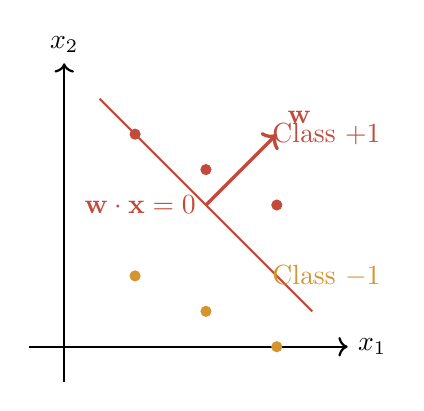
\begin{tikzpicture}[scale=0.9]
    \draw[->, thick] (-0.5,0) -- (4,0) node[right]{$x_1$};
    \draw[->, thick] (0,-0.5) -- (0,4) node[above]{$x_2$};
    \draw[wp-primary, thick] (0.5,3.5) -- (3.5,0.5) node[midway, left]{$\mathbf{w}\cdot\mathbf{x}=0$};
    \draw[->, wp-primary, very thick] (2,2) -- (3,3) node[above right]{$\mathbf{w}$};
    \filldraw[wp-primary] (1,3) circle (2pt);
    \filldraw[wp-primary] (2,2.5) circle (2pt);
    \filldraw[wp-primary] (3,2) circle (2pt);
    \filldraw[wp-accent] (1,1) circle (2pt);
    \filldraw[wp-accent] (2,0.5) circle (2pt);
    \filldraw[wp-accent] (3,0) circle (2pt);
    \node[wp-primary] at (3.7,3) {Class $+1$};
    \node[wp-accent] at (3.7,1) {Class $-1$};
\end{tikzpicture}
\caption{Geometric interpretation of the perceptron: the weight vector $\mathbf{w}$ is orthogonal to the decision hyperplane and points toward the positive class.}
\end{marginfigure}

\paragraph{The XOR Limitation}

The perceptron can represent all primitive Boolean functions (AND, OR, NAND, NOR) because they are linearly separable. However, it fails for the XOR function: $x_1 \oplus x_2 = 1$ iff $x_1 \neq x_2$. Figure~\ref{fig:xor_combined} shows that no single line can separate the points $(0,0)$ and $(1,1)$ from $(1,0)$ and $(0,1)$. This limitation, highlighted by Minsky and Papert in 1969, led to the first “AI winter” and motivated the development of multilayer networks.

\begin{figure}[h]
    \centering
    \begin{subfigure}{0.45\textwidth}
        \centering
        \begin{tabular}{c|c|c}
            $x_1$ & $x_2$ & $x_1 \oplus x_2$ \\ \hline
            0 & 0 & 0 \\
            1 & 0 & 1 \\
            0 & 1 & 1 \\
            1 & 1 & 0
        \end{tabular}
        \caption{XOR truth table}
        \label{tab:xor}
    \end{subfigure}
    \begin{subfigure}{0.45\textwidth}
        \centering
        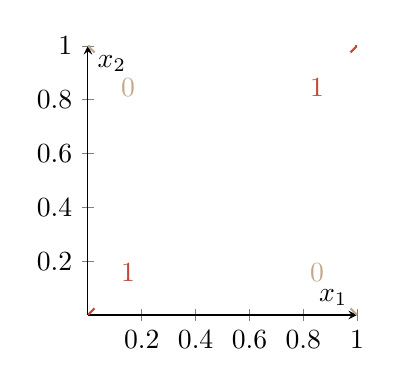
\begin{tikzpicture}
            \tikzstyle{point}=[thick,draw=wp-text,cross out,inner sep=0pt,minimum width=4pt,minimum height=4pt]
            \begin{axis}[axis x line=middle, axis y line=middle, width=5cm, height=5cm, xmin=0, xmax=1, ymin=0, ymax=1, xlabel=$x_1$, ylabel=$x_2$]
                \node[point,label={[label distance=0.3cm,text=wp-muted]135:$0$},wp-muted] at (axis cs:1,0) {};
                \node[point,label={[label distance=0.3cm,text=wp-muted]-45:$0$},wp-muted] at (axis cs:0,1) {};
                \node[point,label={[label distance=0.3cm,text=wp-primary]45:$1$},wp-primary] at (axis cs:0,0) {};
                \node[point,label={[label distance=0.3cm,text=wp-primary]-135:$1$},wp-primary] at (axis cs:1,1) {};
            \end{axis}
        \end{tikzpicture}
        \caption{XOR is not linearly separable}
        \label{fig:xor_plot}
    \end{subfigure}
    \caption{The XOR problem: no single straight line can separate the two classes.}
    \label{fig:xor_combined}
\end{figure}

\subsection{Learning Rules for a Single Unit}

\subsubsection{Perceptron Training Rule}

One way to find an acceptable weight vector is to start with random weights and iteratively update them whenever the perceptron misclassifies an example. The perceptron rule modifies weight $w_i$ (associated with input $x_i$) by
\[
\Delta w_i = \eta\,(t - o)\,x_i,
\]
where $t$ is the target output (0 or 1), $o$ the perceptron’s output, and $\eta \in (0,1)$ the \textbf{learning rate}. This rule converges if the data are linearly separable; otherwise it may oscillate.

\subsubsection{Delta Rule and Gradient Descent}

For non‑separable problems, we need a rule that minimises a continuous error function. Consider a \textbf{linear unit} $o = \mathbf{w}\cdot\mathbf{x}$ (no threshold). Define the sum of squared errors over a training set $\mathcal{D} = \{(\mathbf{x}_d, t_d)\}_{d=1}^N$:
\[
E(\mathbf{w}) = \frac{1}{2}\sum_{d=1}^N (t_d - o_d)^2.
\]
The factor $\frac12$ simplifies differentiation. The gradient of $E$ with respect to $\mathbf{w}$ is
\[
\nabla E(\mathbf{w}) = \sum_{d=1}^N (o_d - t_d)\,\mathbf{x}_d,
\]
so the gradient descent update (batch mode) becomes
\[
\mathbf{w} \leftarrow \mathbf{w} - \eta \nabla E(\mathbf{w}) = \mathbf{w} + \eta \sum_{d=1}^N (t_d - o_d)\,\mathbf{x}_d.
\]

\begin{remark}[Connection to Maximum Likelihood Estimation]
    Assume a regression model $y = \mathbf{w}^{\mathsf{T}}\mathbf{x} + \varepsilon$, with $\varepsilon \sim \mathcal{N}(0,\sigma^2)$. The likelihood of the data is $\prod_{d=1}^N \frac{1}{\sqrt{2\pi\sigma^2}}\exp\!\left(-\frac{(y_d - \mathbf{w}^{\mathsf{T}}\mathbf{x}_d)^2}{2\sigma^2}\right)$. Taking negative logs and discarding constants gives $\frac{1}{2\sigma^2}\sum_d (y_d - \mathbf{w}^{\mathsf{T}}\mathbf{x}_d)^2$. Minimising this is exactly the delta rule (scaled by $1/\sigma^2$). Hence, minimising the squared error is equivalent to maximum likelihood estimation under a Gaussian noise model.
\end{remark}

\subsubsection{Stochastic Gradient Descent (SGD)}

For large $N$, computing the full gradient every iteration is expensive. SGD approximates it using a single randomly chosen example (or a small mini‑batch):
\[
\mathbf{w} \leftarrow \mathbf{w} - \eta \nabla \ell_i(\mathbf{w}),
\]
where $\nabla \ell_i$ is the gradient of the loss for the $i$-th example. The stochasticity introduces noise that can help escape shallow local minima, and the algorithm is the workhorse of deep learning.

\subsection{Activation Functions}

To build multilayer networks, we need nonlinear, differentiable activation functions. Without nonlinearity, stacking linear layers would still produce a linear function. Common choices include:

\begin{defn}[Sigmoid]
    \[
    \sigma(z) = \frac{1}{1+e^{-z}} \in (0,1),\quad \sigma'(z) = \sigma(z)(1-\sigma(z)).
    \]
    Historically popular, but suffers from vanishing gradients for large $|z|$.
\end{defn}
\begin{defn}[Hyperbolic Tangent (tanh)]
    \[
    \tanh(z) = \frac{e^{z}-e^{-z}}{e^{z}+e^{-z}} \in (-1,1),\quad \tanh'(z) = 1-\tanh^2(z).
    \]
    Zero‑centered, which helps optimisation, but still saturates.
\end{defn}
\begin{defn}[Rectified Linear Unit (ReLU)]
    \[
    \text{ReLU}(z) = \max(0,z),\quad \text{ReLU}'(z) = \begin{cases} 1 & \text{if } z>0,\\ 0 & \text{otherwise.} \end{cases}
    \]
    Computationally efficient and mitigates vanishing gradients for positive inputs. May cause “dead neurons” (never activate) if learning rate is too high.
\end{defn}
\begin{defn}[Leaky ReLU / ELU / Swish]
    Variants (e.g., Leaky ReLU: $\max(\alpha z, z)$ with $\alpha \approx 0.01$) address the dying ReLU problem.
\end{defn}

\begin{marginfigure}
\centering
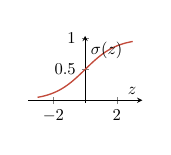
\begin{tikzpicture}[scale=0.6]
    \begin{axis}[width=4cm, height=3cm, xlabel=$z$, ylabel=$\sigma(z)$, domain=-3:3, samples=100, axis lines=middle, enlargelimits]
        \addplot[wp-primary, thick] {1/(1+exp(-x))};
    \end{axis}
\end{tikzpicture}
\caption{The sigmoid activation squashes inputs to $(0,1)$ and is differentiable.}
\end{marginfigure}

\subsection{Multilayer Perceptron and Backpropagation}

A \textbf{multilayer perceptron (MLP)} consists of an input layer, one or more hidden layers, and an output layer. Each neuron in layer $\ell$ receives activations $\mathbf{o}^{(\ell-1)}$ from the previous layer, computes a weighted sum plus bias, and passes it through an activation function. In vectorised form:
\[
\mathbf{a}^{(\ell)} = \mathbf{W}^{(\ell)}\mathbf{o}^{(\ell-1)} + \mathbf{b}^{(\ell)},\qquad 
\mathbf{o}^{(\ell)} = f^{(\ell)}(\mathbf{a}^{(\ell)}),
\]
where $\mathbf{o}^{(0)} = \mathbf{x}$ (the input). The output layer produces $\hat{\mathbf{y}} = \mathbf{o}^{(L)}$.

\subsubsection{Derivation of Backpropagation}

We wish to minimise a loss function $\mathcal{L}(\hat{\mathbf{y}}, \mathbf{t})$ over the training set. For a single example, define the error at the output layer as the derivative of $\mathcal{L}$ with respect to the pre‑activation $\mathbf{a}^{(L)}$:
\[
\boldsymbol{\delta}^{(L)} = \frac{\partial \mathcal{L}}{\partial \mathbf{a}^{(L)}} = \nabla_{\hat{\mathbf{y}}}\mathcal{L} \odot f^{(L)'}(\mathbf{a}^{(L)}),
\]
where $\odot$ denotes elementwise multiplication. For the squared loss $\mathcal{L} = \frac12\|\mathbf{t}-\hat{\mathbf{y}}\|^2$, we have $\nabla_{\hat{\mathbf{y}}}\mathcal{L} = \hat{\mathbf{y}} - \mathbf{t}$.

Now apply the chain rule to propagate the error backwards. For layer $\ell$ (with $\ell < L$), $\mathbf{a}^{(\ell)}$ influences $\mathcal{L}$ through $\mathbf{a}^{(\ell+1)} = \mathbf{W}^{(\ell+1)}\mathbf{o}^{(\ell)} + \mathbf{b}^{(\ell+1)}$ and $\mathbf{o}^{(\ell)} = f^{(\ell)}(\mathbf{a}^{(\ell)})$. Therefore,
\[
\boldsymbol{\delta}^{(\ell)} = \frac{\partial \mathcal{L}}{\partial \mathbf{a}^{(\ell)}} 
= \left( \frac{\partial \mathbf{a}^{(\ell+1)}}{\partial \mathbf{o}^{(\ell)}} \right)^{\mathsf{T}} \frac{\partial \mathcal{L}}{\partial \mathbf{a}^{(\ell+1)}} \odot f^{(\ell)'}(\mathbf{a}^{(\ell)})
= \bigl( (\mathbf{W}^{(\ell+1)})^{\mathsf{T}} \boldsymbol{\delta}^{(\ell+1)} \bigr) \odot f^{(\ell)'}(\mathbf{a}^{(\ell)}).
\]

The gradients with respect to weights and biases are then:
\[
\frac{\partial \mathcal{L}}{\partial \mathbf{W}^{(\ell)}} = \boldsymbol{\delta}^{(\ell)} (\mathbf{o}^{(\ell-1)})^{\mathsf{T}},\qquad
\frac{\partial \mathcal{L}}{\partial \mathbf{b}^{(\ell)}} = \boldsymbol{\delta}^{(\ell)}.
\]

These gradients are used in SGD (or any gradient‑based optimiser) to update the network parameters. The algorithm is summarised below.

\begin{algorithm}[h]
    \caption{Backpropagation (stochastic / mini‑batch version)}
    \textbf{Input:} Training examples $(\mathbf{x}, \mathbf{t})$, learning rate $\eta$, mini‑batch size $m$.
    \textbf{Output:} Trained weights and biases.
    \begin{enumerate}
        \item Initialise all $\mathbf{W}^{(\ell)}$ and $\mathbf{b}^{(\ell)}$ (e.g., using He or Xavier initialisation).
        \item Repeat until convergence:
        \begin{enumerate}
            \item Sample a mini‑batch $\mathcal{B}$ of $m$ examples.
            \item For each example in $\mathcal{B}$, perform forward propagation to compute all $\mathbf{a}^{(\ell)}$ and $\mathbf{o}^{(\ell)}$.
            \item Compute the output error $\boldsymbol{\delta}^{(L)} = \nabla_{\hat{\mathbf{y}}}\mathcal{L} \odot f^{(L)'}(\mathbf{a}^{(L)})$.
            \item For $\ell = L-1$ down to $1$:
                \[
                \boldsymbol{\delta}^{(\ell)} = \bigl((\mathbf{W}^{(\ell+1)})^{\mathsf{T}} \boldsymbol{\delta}^{(\ell+1)}\bigr) \odot f^{(\ell)'}(\mathbf{a}^{(\ell)}).
                \]
            \item Accumulate gradients over the mini‑batch:
                \[
                \frac{\partial \mathcal{L}_{\mathcal{B}}}{\partial \mathbf{W}^{(\ell)}} \leftarrow \frac{1}{m}\sum_{i\in\mathcal{B}} \boldsymbol{\delta}_i^{(\ell)} (\mathbf{o}_i^{(\ell-1)})^{\mathsf{T}},\quad
                \frac{\partial \mathcal{L}_{\mathcal{B}}}{\partial \mathbf{b}^{(\ell)}} \leftarrow \frac{1}{m}\sum_{i\in\mathcal{B}} \boldsymbol{\delta}_i^{(\ell)}.
                \]
            \item Update parameters: $\mathbf{W}^{(\ell)} \leftarrow \mathbf{W}^{(\ell)} - \eta \frac{\partial \mathcal{L}_{\mathcal{B}}}{\partial \mathbf{W}^{(\ell)}}$, similarly for $\mathbf{b}^{(\ell)}$.
        \end{enumerate}
    \end{enumerate}
\end{algorithm}

\subsection{Advanced Optimisation Methods}

Plain SGD can be slow or sensitive to learning rate choices. Modern deep learning often uses improved optimisers:

\begin{itemize}
    \item \textbf{Momentum}: maintains a velocity vector $\mathbf{v}_t = \gamma \mathbf{v}_{t-1} + \eta \nabla \mathcal{L}$, then updates parameters by $\mathbf{w} \leftarrow \mathbf{w} - \mathbf{v}_t$. This dampens oscillations and accelerates convergence.
    \item \textbf{Adam (Adaptive Moment Estimation)}: maintains per‑parameter learning rates using exponentially decaying averages of gradients and squared gradients. It is robust and widely used.
    \item \textbf{Learning rate scheduling}: reducing the learning rate over time (e.g., step decay, cosine annealing, or warmup) helps the model fine‑tune towards a minimum.
\end{itemize}

\subsection{Regularisation for Neural Networks}

Deep networks have many parameters and can easily overfit. Several techniques reduce overfitting:

\subsubsection{L2 Regularisation (Weight Decay)}
Add a penalty $\frac{\lambda}{2}\|\mathbf{w}\|_2^2$ to the loss. This encourages small weights and corresponds to a Gaussian prior on $\mathbf{w}$ in a Bayesian (MAP) framework.

\subsubsection{Dropout}
During training, randomly set a fraction $p$ of neurons (and their connections) to zero at each forward pass. This prevents co‑adaptation and can be interpreted as training an ensemble of thinned networks. At test time, all neurons are used but their outputs are scaled by $p$.

\subsubsection{Batch Normalisation (BatchNorm)}
For each mini‑batch, BatchNorm normalises the pre‑activations to have zero mean and unit variance, then applies a learned scale $\gamma$ and shift $\beta$:
\[
\mu_{\mathcal{B}} = \frac{1}{m}\sum_{i\in\mathcal{B}} a_i,\quad \sigma_{\mathcal{B}}^2 = \frac{1}{m}\sum_{i\in\mathcal{B}} (a_i-\mu_{\mathcal{B}})^2,\quad \hat{a}_i = \frac{a_i-\mu_{\mathcal{B}}}{\sqrt{\sigma_{\mathcal{B}}^2+\epsilon}},\quad \tilde{a}_i = \gamma\hat{a}_i+\beta.
\]
BatchNorm accelerates training and acts as a regulariser.

\subsubsection{Early Stopping}
Monitor the validation error during training and stop when it stops improving. This limits the effective capacity and is one of the simplest regularisation methods.

\subsection{Bias–Variance Tradeoff in Neural Networks}

Recall from statistical learning the bias–variance decomposition (for squared loss):
\[
\mathbb{E}_{\mathcal{D}}[R(h_{\mathcal{D}})] = \underbrace{(\mathbb{E}_{\mathcal{D}}[h_{\mathcal{D}}] - h^*)^2}_{\text{bias}^2} + \underbrace{\mathbb{V}_{\mathcal{D}}[h_{\mathcal{D}}]}_{\text{variance}} + \text{noise}.
\]
In neural networks, the model capacity increases with the number of layers and neurons. Low capacity leads to high bias (underfitting); high capacity leads to low bias but high variance (overfitting). Regularisation and early stopping control the effective capacity, trading bias against variance. The optimal capacity is problem‑dependent and is usually found via cross‑validation.

\begin{marginfigure}
\centering
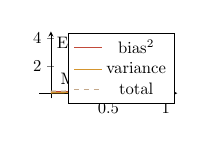
\begin{tikzpicture}[scale=0.6]
    \begin{axis}[width=4.5cm, height=3cm, xlabel=Model capacity, ylabel=Error, domain=0:1, samples=50, axis lines=middle, enlargelimits]
        \addplot[wp-primary, thick] {0.1 + 0.5*(x-0.2)^2};
        \addplot[wp-accent, thick] {0.5*exp(5*(x-0.6))};
        \addplot[wp-muted, thick, dashed] {0.1 + 0.5*(x-0.2)^2 + 0.5*exp(5*(x-0.6))};
        \legend{bias$^2$, variance, total};
    \end{axis}
\end{tikzpicture}
\caption{Typical bias–variance tradeoff: total generalisation error has a minimum at the optimal capacity.}
\end{marginfigure}

\subsection{Universal Approximation Theorem}

One of the most important theoretical results for neural networks is the universal approximation theorem.

\begin{thm}[Cybenko, 1989]
    Let $\sigma: \mathbb{R}\to\mathbb{R}$ be any continuous, bounded, non‑constant activation function (e.g., sigmoid). Then for any continuous function $f: [0,1]^d \to \mathbb{R}$ and any $\varepsilon > 0$, there exist an integer $N$, vectors $\mathbf{w}_j \in \mathbb{R}^d$, scalars $v_j, b_j \in \mathbb{R}$ such that
    \[
    \sup_{\mathbf{x}\in[0,1]^d} \left| \sum_{j=1}^{N} v_j \, \sigma(\mathbf{w}_j\cdot\mathbf{x} + b_j) - f(\mathbf{x}) \right| < \varepsilon.
    \]
\end{thm}

The theorem implies that a single hidden layer (with enough neurons) can approximate any continuous function arbitrarily well. However, it does not guarantee that such a network can be learned efficiently; the required number of neurons $N$ may be astronomically large. Deep networks (many layers) can represent certain functions exponentially more compactly than shallow ones, which is the main motivation for deep learning.

Figure~\ref{fig:UAT_fixed} illustrates the idea: approximating $\sin(x)$ with piecewise linear functions (which can be built from ReLU units). As the number of linear regions increases (i.e., as we add more hidden units), the approximation improves.

\begin{figure}[h]
\centering
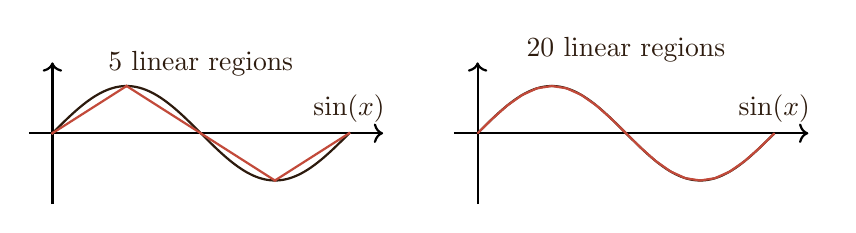
\begin{tikzpicture}[scale=.6, thick]
    % First plot: 5 linear regions
    \begin{scope}[shift={(0, 0)}]
        \draw[->] (-0.5,0) -- (7,0) node[right] {};
        \draw[->] (0,-1.5) -- (0,1.5) node[above] {};
        \draw[wp-text, thick, domain=0:6.28, samples=100, smooth] plot (\x, {sin(\x r)});
        \draw[wp-primary, thick] (0,0) -- (1.57,1);
        \draw[wp-primary, thick] (1.57,1) -- (3.14,0);
        \draw[wp-primary, thick] (3.14,0) -- (4.71,-1);
        \draw[wp-primary, thick] (4.71,-1) -- (6.28,0);
        \node[above] at (6.28,0) {\textcolor{wp-text}{$\sin(x)$}};
        \node[above] at (3.14,1) {\textcolor{wp-text}{5 linear regions}};
        \foreach \x/\y in {0/0, 1.57/1, 3.14/0, 4.71/-1, 6.28/0} \fill[wp-primary] (\x,\y) circle (1pt);
    \end{scope}
    % Second plot: 20 linear regions
    \begin{scope}[shift={(9,0)}]
        \draw[->] (-0.5,0) -- (7,0) node[right] {};
        \draw[->] (0,-1.5) -- (0,1.5) node[above] {};
        \draw[wp-text, thick, domain=0:6.28, samples=100, smooth] plot (\x, {sin(\x r)});
        \foreach \i in {0,...,19} {
            \pgfmathsetmacro{\xstart}{\i * 6.28 / 20}
            \pgfmathsetmacro{\xend}{(\i + 1) * 6.28 / 20}
            \pgfmathsetmacro{\ystart}{sin(\xstart r)}
            \pgfmathsetmacro{\yend}{sin(\xend r)}
            \draw[wp-primary, thick] (\xstart, \ystart) -- (\xend, \yend);
        }
        \node[above] at (6.28,0) {\textcolor{wp-text}{$\sin(x)$}};
        \node[above] at (3.14,1.3) {\textcolor{wp-text}{20 linear regions}};
        \foreach \i in {0,...,20} {
            \pgfmathsetmacro{\x}{\i * 6.28 / 20}
            \pgfmathsetmacro{\y}{sin(\x r)}
            \fill[wp-primary] (\x,\y) circle (0.5pt);
        }
    \end{scope}
\end{tikzpicture}
\caption{Approximating $\sin(x)$ with piecewise linear functions (e.g., ReLU networks). More hidden units (more linear regions) yield a better approximation, illustrating the universal approximation theorem.}
\label{fig:UAT_fixed}
\end{figure}

\subsection{Weight Initialisation}

Proper initialisation is crucial for deep networks to avoid vanishing or exploding gradients. Two widely used schemes are:

\begin{itemize}
    \item \textbf{Xavier (Glorot) initialisation}: for tanh or sigmoid, set $\text{Var}[w] = \frac{2}{n_{\text{in}} + n_{\text{out}}}$, where $n_{\text{in}}$ and $n_{\text{out}}$ are the numbers of input and output units of the layer.
    \item \textbf{He (Kaiming) initialisation}: for ReLU, set $\text{Var}[w] = \frac{2}{n_{\text{in}}}$.
\end{itemize}

These choices keep the signal variance roughly constant across layers, promoting stable gradient flow.

With these foundations – perceptron, gradient descent, backpropagation, activation functions, optimisation, regularisation, bias–variance tradeoff, universal approximation, and initialisation – we have a rigorous yet intuitive understanding of how neural networks learn. Subsequent chapters will build on these ideas to introduce convolutional networks, recurrent networks, and generative models.
\end{document}
